%% generated by gen_tables.py -- do not edit
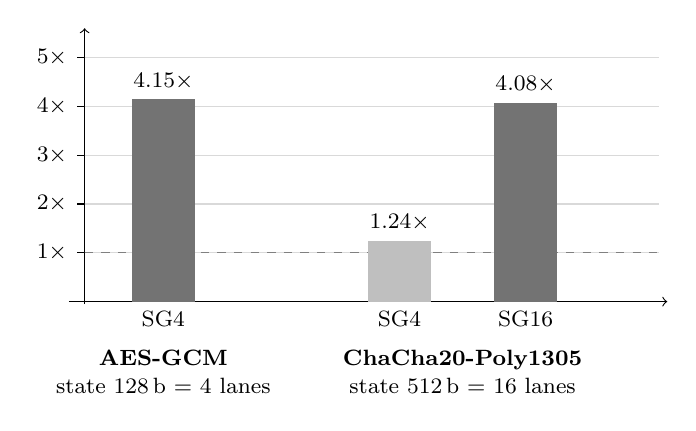
\begin{tikzpicture}[x=1cm,y=0.62cm, font=\footnotesize]
  \draw[->] (-0.2,0) -- (7.4,0) node[below left]{};
  \draw[->] (0,-0.05) -- (0,5.6*1) ;
  \foreach \y in {1,2,3,4,5} {
    \draw (0,\y) -- (-0.1,\y) node[left]{\y$\times$};
    \draw[gray!30] (0,\y) -- (7.3,\y); }
  \draw[dashed,gray] (0,1) -- (7.3,1);
  %% AES-GCM: state 128 b = 4 lanes
  \fill[black!55] (0.6,0) rectangle +(0.8,4.146);
  \node[above] at (1.0,4.146) {4.15$\times$};
  \node[below] at (1.0,0) {SG4};
  \node[below=14pt] at (1.0,0) {\textbf{AES-GCM}};
  \node[below=24pt] at (1.0,0) {state 128\,b $=$ 4 lanes};
  %% ChaCha: state 512 b = 16 lanes
  \fill[black!25] (3.6,0) rectangle +(0.8,1.242);
  \node[above] at (4.0,1.242) {1.24$\times$};
  \node[below] at (4.0,0) {SG4};
  \fill[black!55] (5.2,0) rectangle +(0.8,4.076);
  \node[above] at (5.6,4.076) {4.08$\times$};
  \node[below] at (5.6,0) {SG16};
  \node[below=14pt] at (4.8,0) {\textbf{ChaCha20-Poly1305}};
  \node[below=24pt] at (4.8,0) {state 512\,b $=$ 16 lanes};
\end{tikzpicture}
